%=====================================================================
\section{Method}
% =====================================================================

The automated migration system operates as a nightly pipeline with
three main stages, illustrated conceptually in
Figure~\ref{fig:overview}, which repeats until no unresolved
references to a given identifier remain.

\begin{figure}
  \centering
  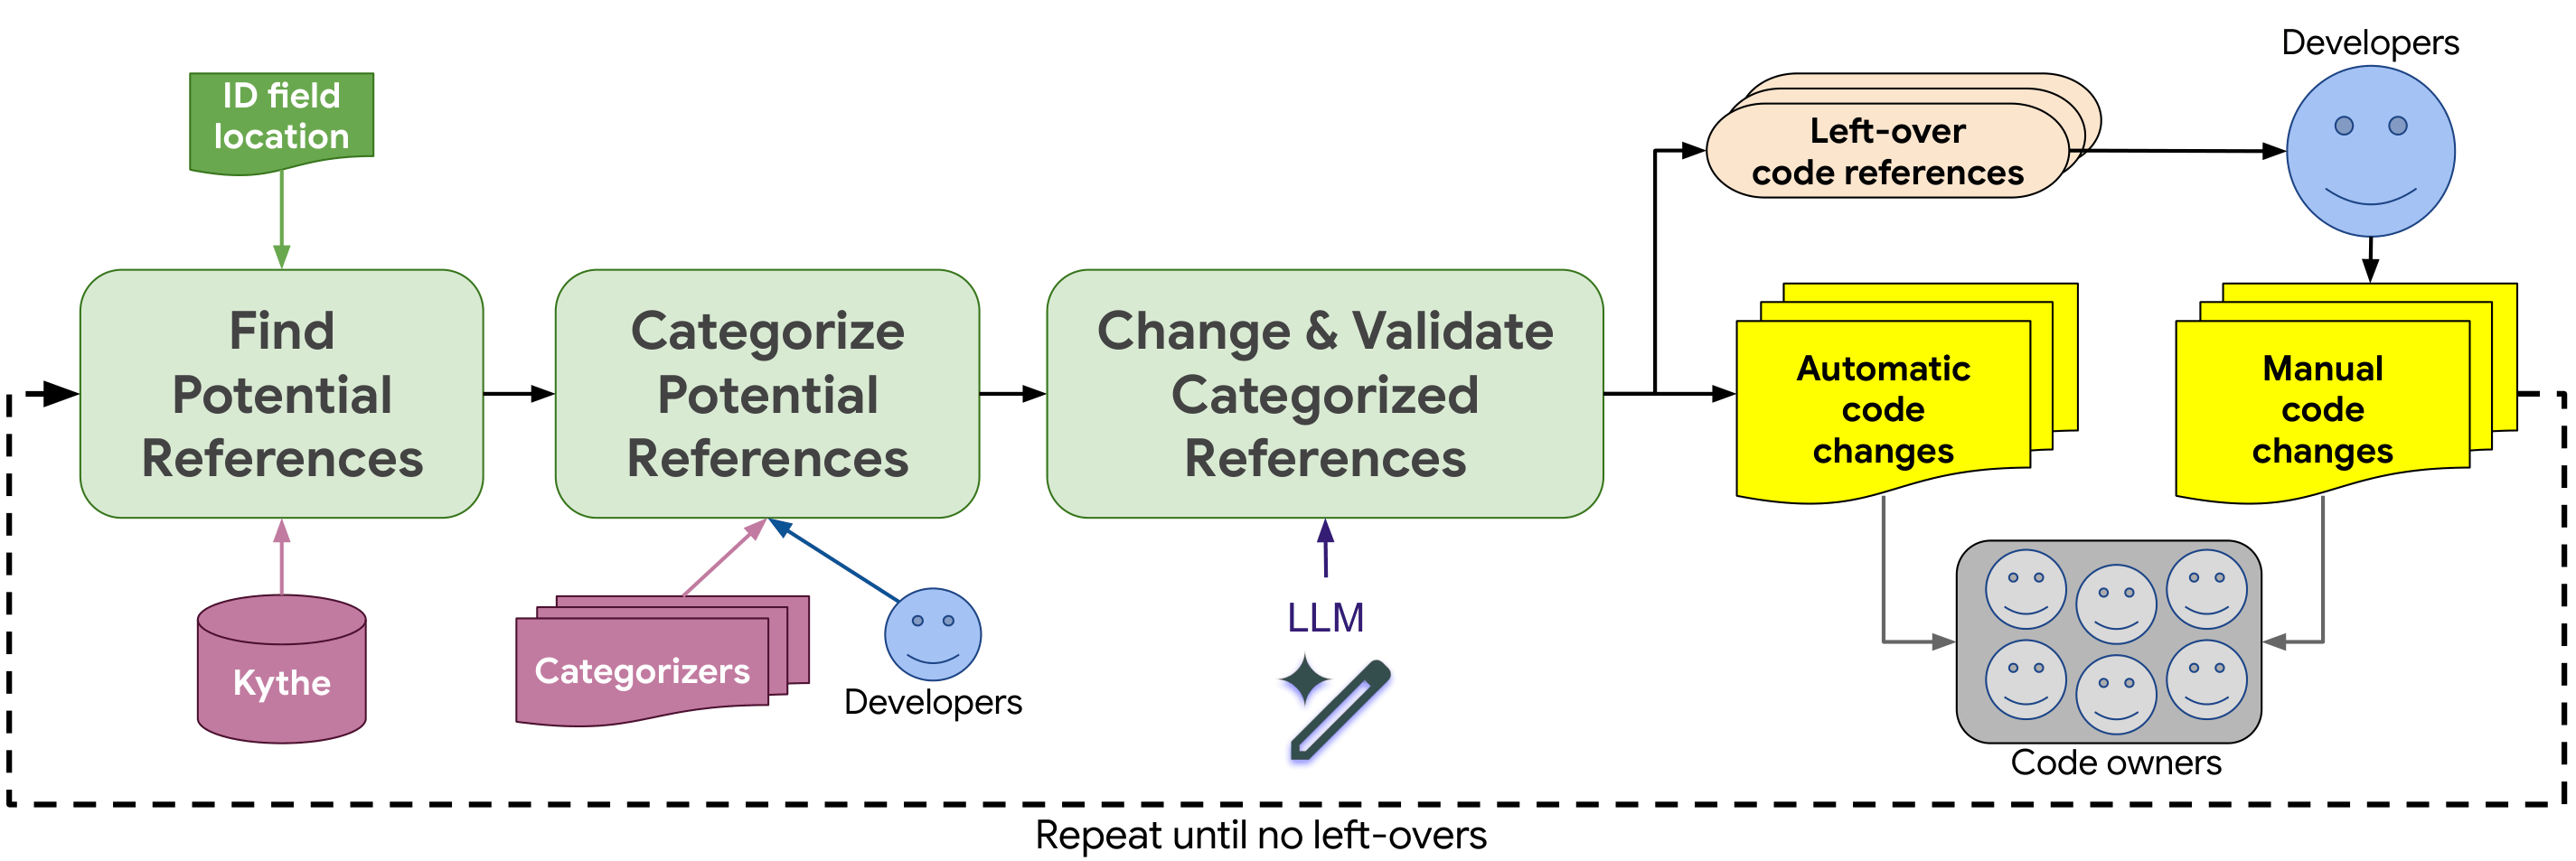
\includegraphics[width=0.8\linewidth]{system-overview.png}
  \caption{High-level overview of the automated migration pipeline
  (screenshot of Figure~1 from the original paper).}
  \label{fig:overview}
\end{figure}

\subsection{Motivating Example Walkthrough}
Before describing each pipeline stage in detail, it helps to ground
all three in a concrete scenario. Suppose a schema field identifying
items in an inventory system is declared as a 32-bit integer, and the
owning team decides to widen it to 64 bits because the item count is
approaching the 32-bit limit. A minimal, adapted illustration of the
kind of code this touches is shown below (this is an original,
simplified stand-in for the style of example used in the paper, not a
reproduction of it):

\begin{Verbatim}[frame=single, framesep=5pt, numbers=left, numbersep=3pt, fontsize=\footnotesize]
int itemId = record.getItemId();
boolean isLegacy = ((itemId >> 31) == 1);

// test code
Record r = Record.newBuilder()
  .setItemId(-7)
  .build();
\end{Verbatim}

Three things happen once the field's declared type changes. First,
the local variable's declared type (\texttt{int}) must widen to match
the field's new accessor return type, or the code will no longer
compile. Second, a bit-shift by 31 that made sense for a 32-bit value
must become a shift by 63 to keep selecting the same high-order bit
on a 64-bit value, a change that a naive text search for the field
name alone would never catch, since the number 31 is not a reference
to the field at all. Third, small hard-coded test values such as
\texttt{-7} technically still compile after the type change but no
longer exercise the new, much larger value range, so tests should
ideally be updated to use identifiers outside the old 32-bit range in
order to catch width-related bugs.

This is exactly the mix of \emph{direct} references (the field
accessor calls), \emph{indirect} references reachable only through
data or control flow (the bit-shift amount), and \emph{semantically
still-valid but no-longer-meaningful} code (the small test literal)
that makes this migration hard to fully automate with text-based
tools alone. It's also what motivates handing the actual editing step
to an LLM that can read and reason about a whole file rather than
matching isolated lines.



\begin{figure}
  \centering
  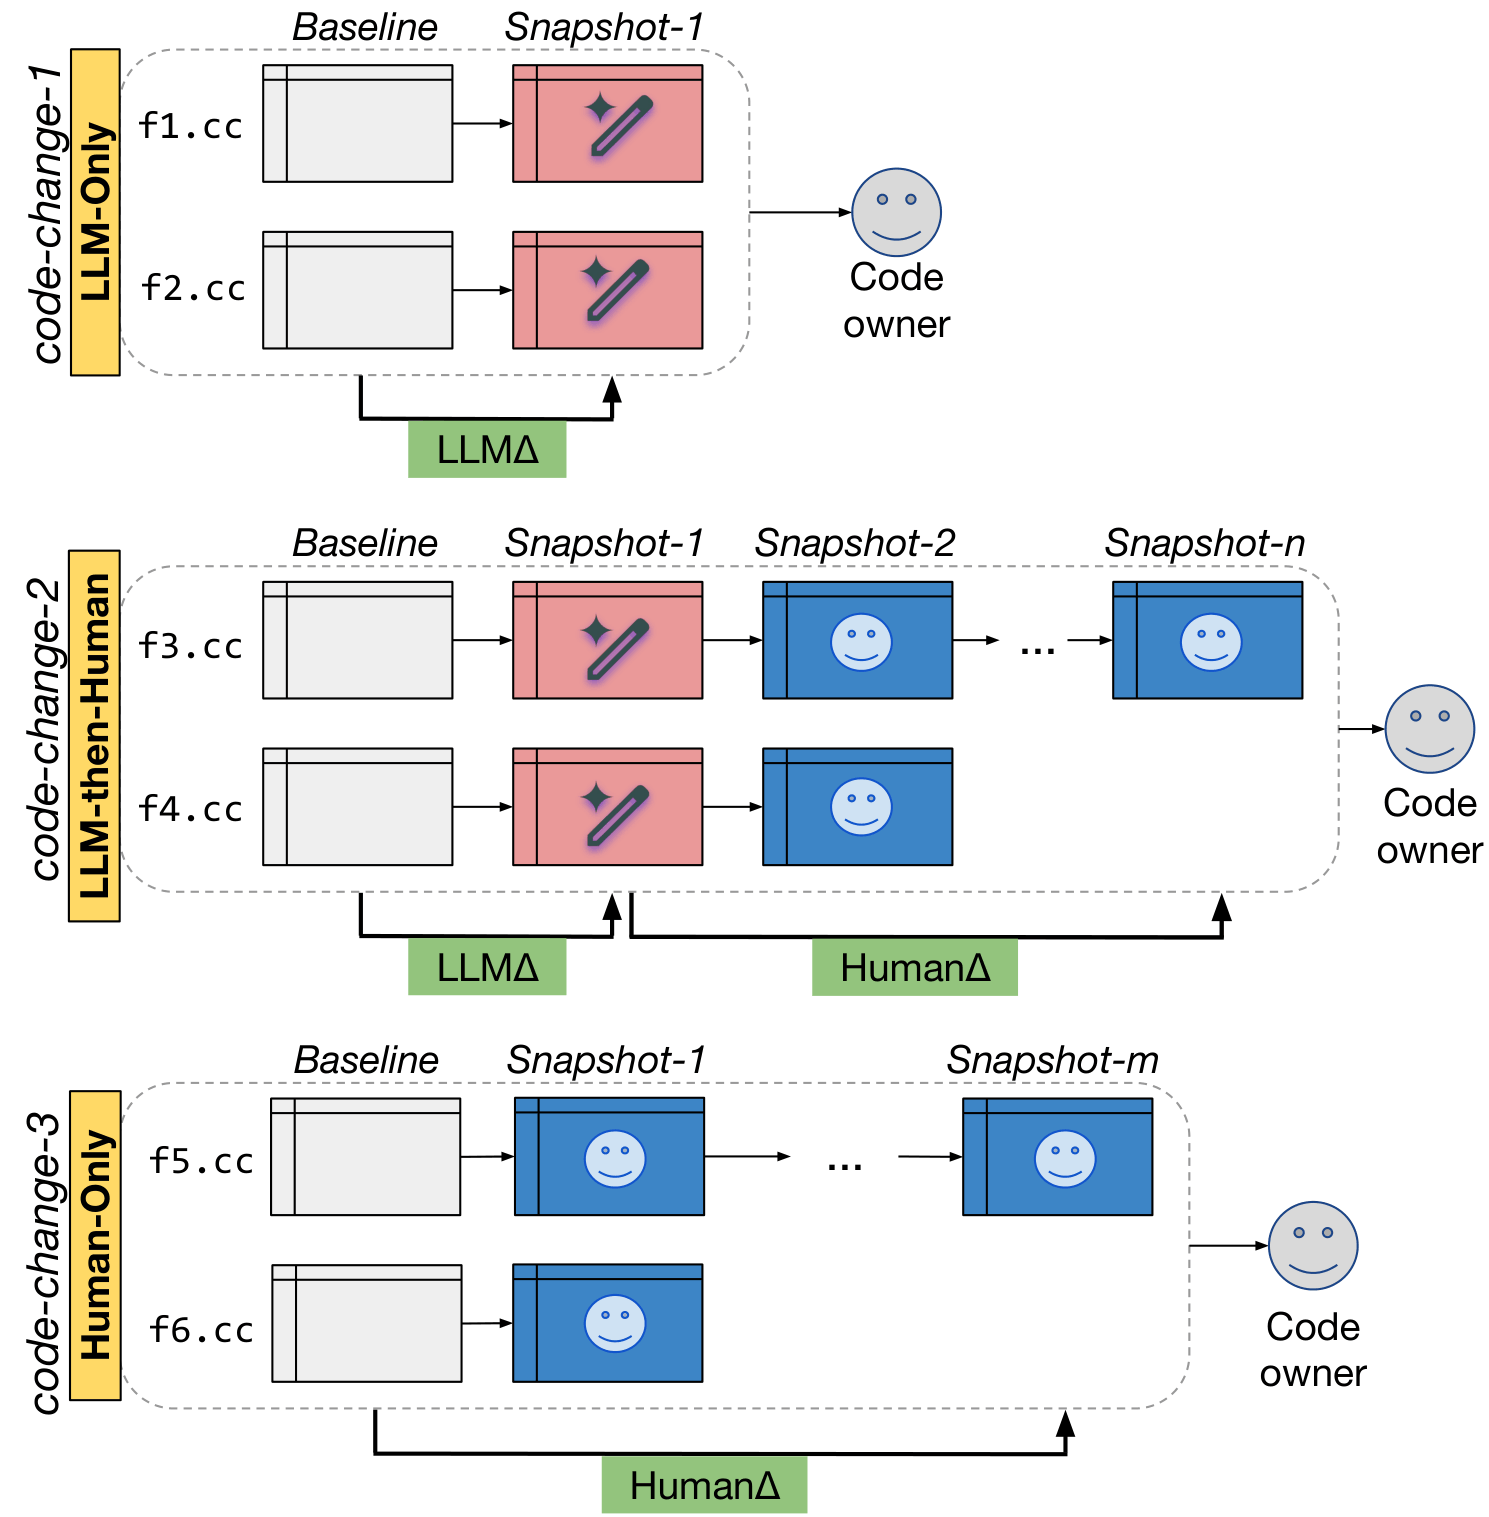
\includegraphics[width=0.8\linewidth]{code-change-types.png}
  \caption{The three code-change categories used to attribute edits
  to the LLM versus to developers (screenshot of Figure~3 from the
  original paper).}
  \label{fig:changetypes}
\end{figure}

Given the location of an identifier field, the system uses Kythe to
find all direct references to it, then recursively expands outward to
indirect references, up to a fixed maximum distance of five hops.
This deliberately produces a superset of the locations that actually
need to change: some flagged locations turn out to be irrelevant
(false positives), and, because the search distance is capped for
practical reasons, some true references beyond five hops may be
missed (false negatives). The authors argue this is an acceptable
trade-off, since more precise techniques such as full data-flow
analysis or AST-based static analysis would be prohibitively expensive
to build and maintain across a codebase written by thousands of
engineers in many languages and styles.

\subsection{Stage 2: Categorizing References}
Each discovered location is run through a bank of lightweight
categorizers, mostly simple regex- and value-range-based heuristics,
that sort it into one of four buckets: \emph{not-migrated} (clearly
still needs updating, high confidence), \emph{irrelevant} (clearly
does not need updating, e.g., a class definition rather than a usage
site), \emph{relevant} (ambiguous, needs closer inspection), or
\emph{left-over} (not confidently classified, queued for manual
developer triage). Developers who investigate left-over locations can
permanently reclassify them via configuration, which the system
consults on subsequent nightly runs.

\subsection{Stage 3: LLM-Driven Change and Validation}
Locations placed in the not-migrated and relevant buckets are handed
to the fine-tuned LLM together with the entire contents of the
containing file and a short natural-language instruction describing
the intended change (e.g., ``update this identifier to a 64-bit type,
and use larger sample values in tests''). The model returns a diff,
applied back onto the original file with a fuzzy diffing algorithm
that tolerates small positional errors in the model's output. Because
model output is non-deterministic even at a fixed temperature, three
independent generation attempts are made per file, and one successful
attempt is chosen at random.

Every LLM-produced change is passed through an ordered chain of
validators, cheapest first, so expensive checks only run on
candidates that already survived the cheap ones. Algorithm~\ref{alg:validation}
summarizes the ordering: a change is discarded (and routed to a human
for manual handling) as soon as it fails any single check.

\begin{algorithm}
\caption{Simplified change-validation pipeline based on Section 3.3 of the original paper.}
\label{alg:validation}
\begin{algorithmic}[1]
\Require candidate file edit produced by the LLM
\If{LLM call did not return successfully}
  \State \Return \textsc{invalid}
\ElsIf{only whitespace/formatting changed}
  \State \Return \textsc{invalid}
\ElsIf{result fails to parse, or AST is unchanged}
  \State \Return \textsc{invalid}
\ElsIf{LLM, when asked, says the change was unnecessary}
  \State \Return \textsc{invalid}
\ElsIf{project fails to build with the change}
  \State \Return \textsc{invalid}
\ElsIf{regression tests fail because of the change}
  \State \Return \textsc{invalid}
\Else
  \State \Return \textsc{ready for review}
\EndIf
\end{algorithmic}
\end{algorithm}

Files that pass every validation step are grouped into code changes
(potentially spanning several files), visually reviewed by the
responsible developer, and sent to the owning team for final approval
and submission through Critique. Figure~\ref{fig:diff} shows, at a
conceptual level, what such a reviewed change looks like inside
Critique's diff view once a file has been edited.


\begin{figure}
  \centering
  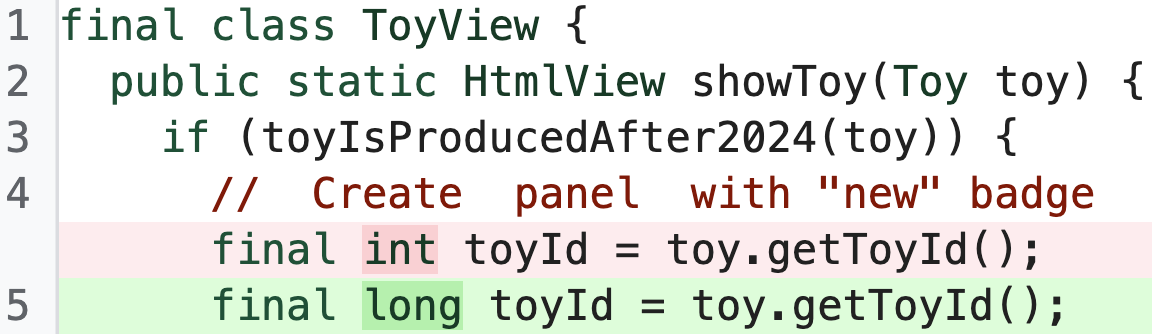
\includegraphics[width=0.75\linewidth]{code-diff.png}
  \caption{Example of a reviewed file edit as it appears in Critique's
  diff view (screenshot of Figure~2 from the original paper).}
  \label{fig:diff}
\end{figure}

\subsection{Prompting Strategy and Observed Edit Patterns}
The natural-language instruction sent to the model alongside a file
is deliberately short and generic rather than file-specific. It
states that the identifier's declared type should change and that
references to it should be updated accordingly, and separately asks
that test code use identifier values large enough to fall outside the
old, narrower range (while keeping the sign of existing negative test
values unchanged). The same wording, translated only insofar as
language-specific accessor-method conventions differ, was reused
across every supported language rather than being hand-tuned per
file.

The authors highlight several qualitative patterns in how the model
responded to this prompt across many files: it reused the same
instruction to correctly update both Java and C++ files despite their
different syntax; it picked the type-appropriate accessor method for
a given language; when a numeric identifier also appeared inside an
embedded SQL query string, it updated both consistently; and, when
given several candidate line numbers containing ambiguous numeric
literals, it could infer which variable was actually the identifier
and edit only that line, rather than blindly changing every suggested
one (Figure~\ref{fig:editexamples}). Developers viewed this
flexibility, handling many languages and edge cases from one generic
instruction, as one of the clearest advantages of an LLM-based
approach over hand-written, per-language transformation rules.


\begin{figure}
  \centering
  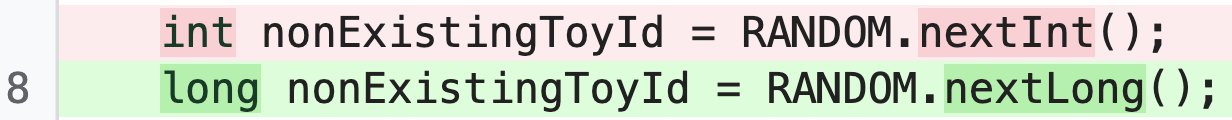
\includegraphics[width=0.7\linewidth]{sample-language-context.png}
  \caption{Examples of qualitative LLM edit behavior observed across
  files and languages (screenshot of Figure~5 from the original
  paper).}
  \label{fig:editexamples}
\end{figure}

\subsection{Evaluation Metrics}
\label{sec:evalmetrics}
To quantify how much of the resulting code was actually written by
the LLM versus by a human, the authors define two metrics based on
Levenshtein edit distance between successive saved snapshots of a
file: \textbf{LLM$\Delta$}, the edit distance between the untouched
baseline and the first LLM-produced snapshot, and
\textbf{Human$\Delta$}, the edit distance between that first snapshot
and the final, human-adjusted snapshot actually submitted. Every
submitted code change is additionally labeled as \emph{LLM-Only}
(entirely from the LLM), \emph{LLM-then-Human} (the LLM produced an
initial version that a developer edited further), or \emph{Human-Only}
(the LLM was not involved at all).
